\chapter{ggplot2}
\section{Introduction}

Have you ever wanted to create interesting, easy-to-read graphics?
Do you enjoy colors and see the value in using them to enhance the appearance of your charts?
Do you enjoy coding?
Then you have come to the right chapter!
This chapter is dedicated to ggplot2, an R package that is used to create visually appealing graphics that take the hassle out of plotting, such as making legends and organization axes. \cite{ggplot2}
ggplot2 can be used to make a wide range of graphics, to the most simple scatter plots to complex maps and charts that contain multiple layers.
Listed below are a few useful commands that we will use throughout this chapter:

\begin{enumerate}
\item \texttt{aes}: define aesthetic mappings
\item \texttt{geom\_area}: ribbons and area plots
\item \texttt{geom\_point}: points, as for scatterplots
\item \texttt{scale\_fill\_discrete}: choses colors evenly spaced around the color wheel; same as hue
\item \texttt{scale\_fill\_gradient} or \texttt{scale\_colour\_gradient}: gradient between two colors
\item \texttt{scale\_fill\_gradient2 or scale\_colour\_gradient2}: gradient with a midpoint color and two colors that diverge from it
\item \texttt{scale\_fill\_gradientn or scale\_colour\_gradientn}: gradient with n colors spaced evenly
\item \texttt{group}: grouping variable for a polygon
\item \texttt{order}: order to connect each point in a group
\item \texttt{region}: generally the names of countries, though sometimes other objects like lakes are also included
\end{enumerate}

\section{Objectives of the Case Study}

In this study, you will learn some useful techniques for displaying different types of variables, including discrete and continuous variables, using various coloring methods.
The first two objectives cover the basics of these methods, while the third objective adds another small level of complexity to the techniques of the first two exercises.

\begin{enumerate}
\item Your first task is to create a graph of a population's age over time where each age group, the discrete variable, is depicted by a different color. You will also design a scatterplot with a gradient that contains a discrete variable.

\item Next, you will learn to color data points on a gradient scale, where the colors represent a continuous variable.

\item Finally, you will finish this chapter by creating a chloropleth map based on variables from a dataset.
\end{enumerate}

\section{Building the Model}

After you have copied and pasted the student code into a new R script, begin by retrieving some data.
You can use the data sets included in the example or find your own via the datasets package or gcookbook package.\medskip

For objective one, the procedure is relatively straightforward.
Depending on the dataset you use, your graph should look something like the graph in Figure \ref{fig:popagebase}.
As you progress through the exercise for the first example, you will be able to change the colors included in the graph and legend.
The basic layout will be the same, but you will be able to change the gradients.

\begin{figure}[htbp!]
   \centering
      \caption{US Population by Age Group - Discrete Variable Mapping}
   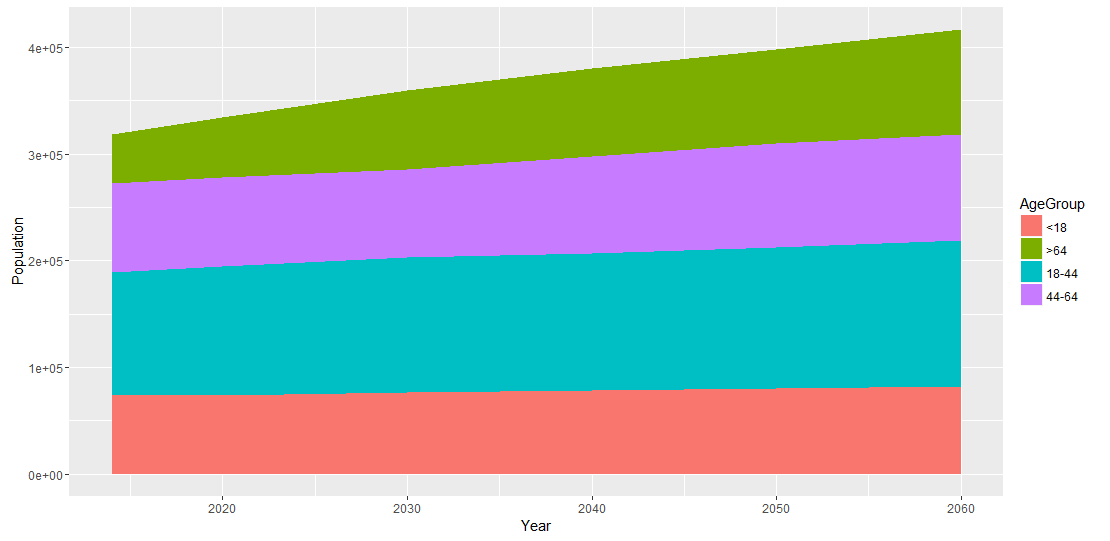
\includegraphics[width=.5\textwidth]{pictures/ggplot2/popagebase.png} 
   \label{fig:popagebase}
\end{figure} 

\noindent Figure \ref{fig:mice.base} has the same basic premise, but this time you will be graphing points on a scatterplot.
Again, you can change the colors that correspond to gender to suit your needs.

\begin{figure}[htbp!]
   \centering
      \caption{Discrete Variable Scatterplots with Mice Data}
   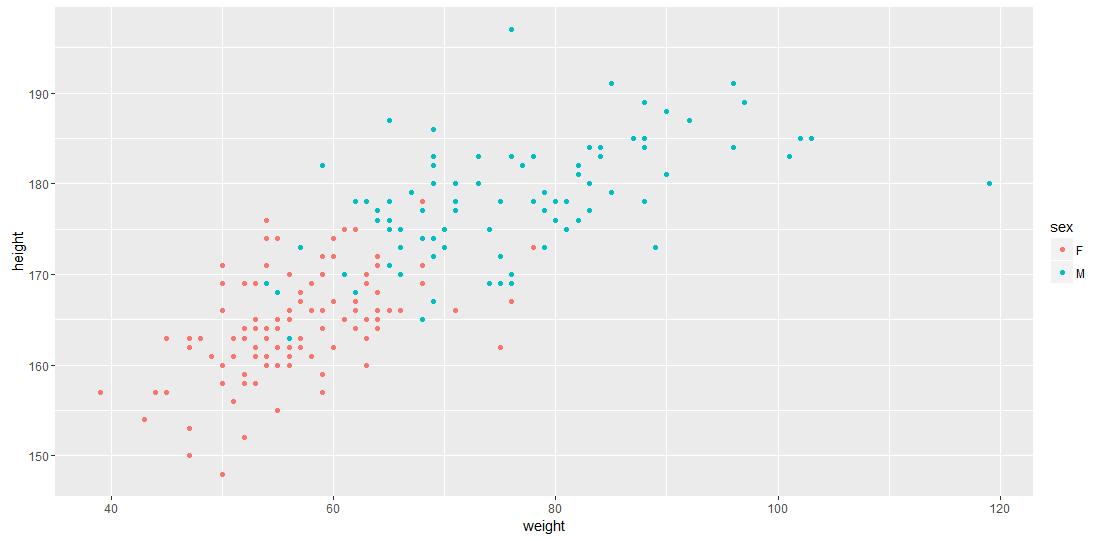
\includegraphics[width=.5\textwidth]{pictures/ggplot2/micebase.png} 
   \label{fig:mice.base}
\end{figure} 

\noindent As we move on to Objective 2, notice the change in coding language from discrete to continuous variables.
To create graphs using discrete variables, we used \texttt{scale\_fill} along with a specific color command, such as \texttt{hue} or \texttt{brewer}.
For graphs that include continuous variables, however, we will add some version of "gradient" to the end of our color commands.
\texttt{Gradient} still allows us to specify which colors we want to use, but it is only for continuous data.\medskip

Go ahead, try creating a scatterplot and changing the colors. Your results should look something like figures \ref{fig:contscatterbase} through \ref{fig:contscatter}.\medskip


\begin{figure}[htbp!]
\centering
\begin{minipage}{.5\textwidth}
  \centering
  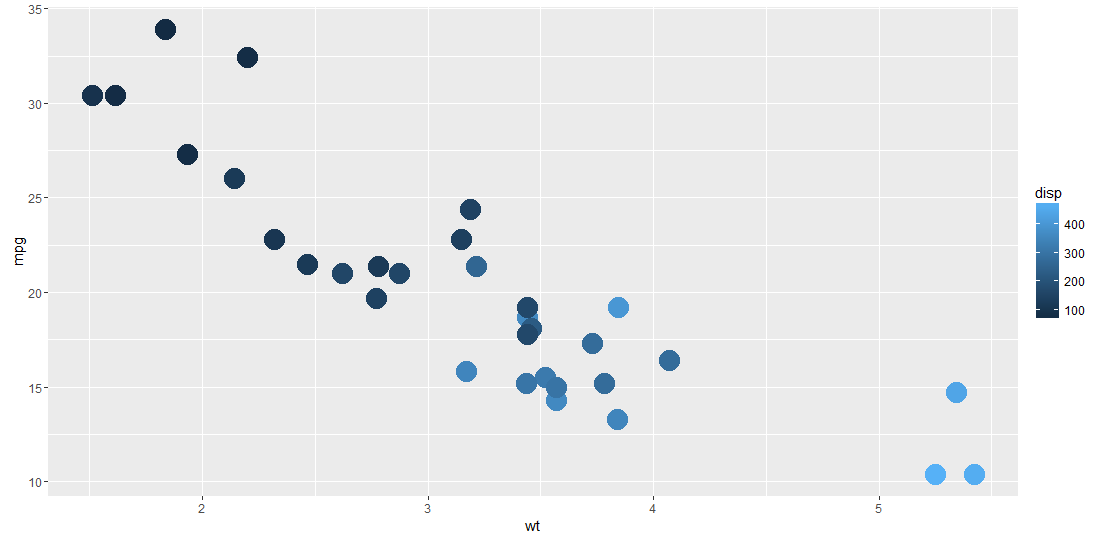
\includegraphics[width=.5\textwidth]{pictures/ggplot2/contscatterbase.png}
  \caption{Base Plot}
  \label{fig:contscatterbase}
\end{minipage}%
\begin{minipage}{.5\textwidth}
  \centering
  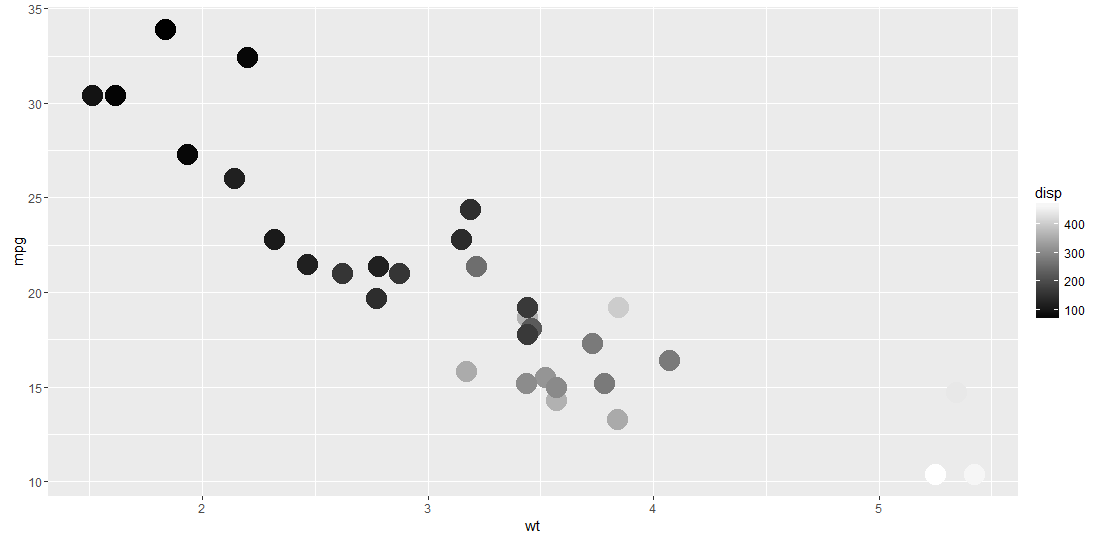
\includegraphics[width=.5\textwidth]{pictures/ggplot2/contscattergrey.png}
  \caption{Plot Using gradient}
  \label{fig:contscattergrey}
\end{minipage}
\end{figure}

\begin{figure}[htbp!]
\centering
\begin{minipage}{.5\textwidth}
  \centering
  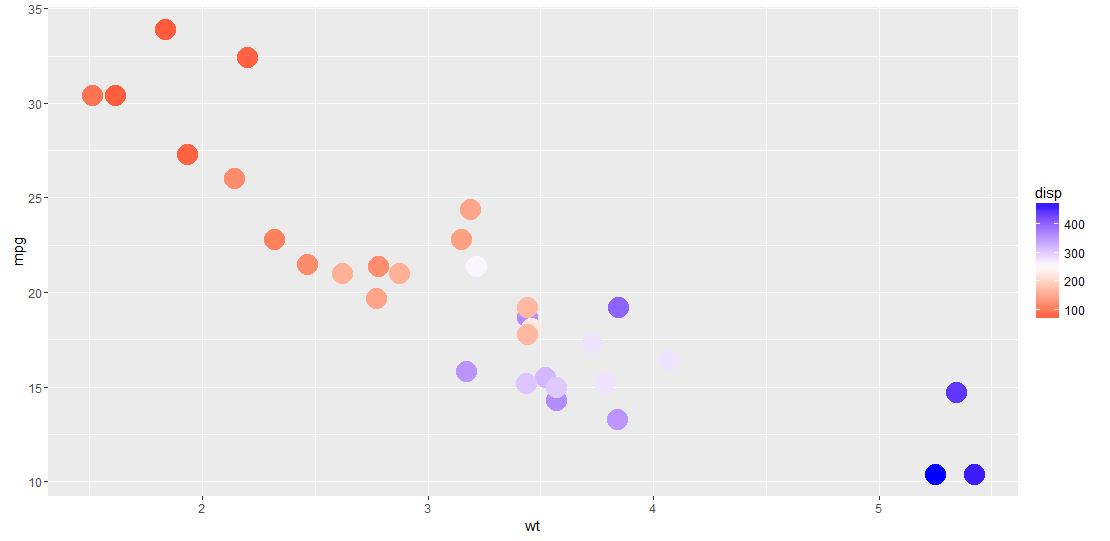
\includegraphics[width=.25\textwidth]{pictures/ggplot2/contscattermidpoint.png}
  \caption{Plot Using gradient2}
  \label{fig:contscattermidpoint}
\end{minipage}%
\begin{minipage}{.5\textwidth}
  \centering
  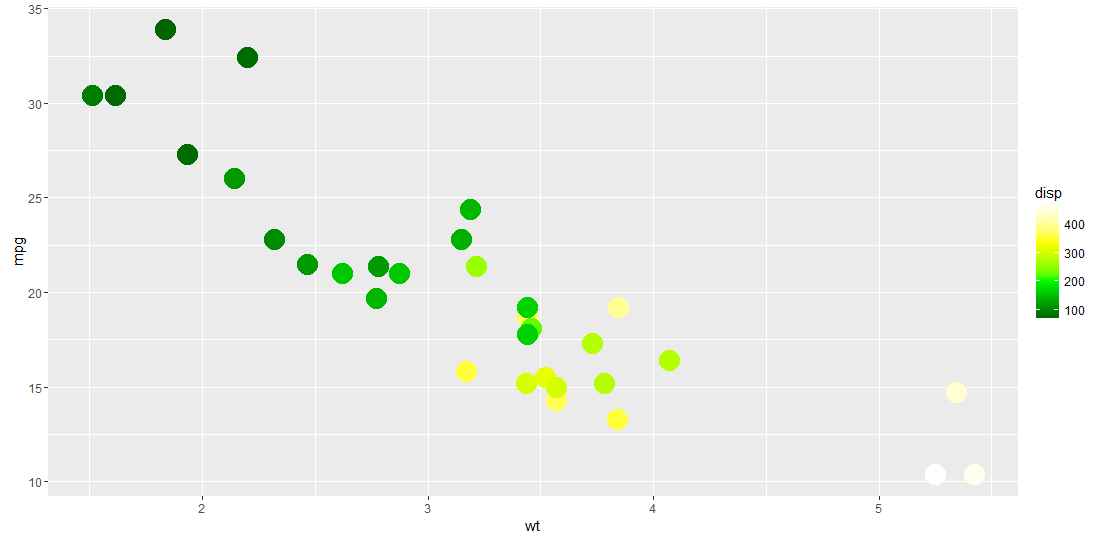
\includegraphics[width=.25\textwidth]{pictures/ggplot2/contscatter.png}
  \caption{Plot Using gradientn}
  \label{fig:contscatter}
\end{minipage}
\end{figure}

\noindent Now that you mastered that concept, let's move on to some plots from Objective 3...

\noindent If you are using the code directly from the student example code, you should first create a  plot that looks a bit like figure \ref{fig:plainUSAmap}.

\begin{figure}[htbp!]
   \centering
      \caption{Plain USA Map}
   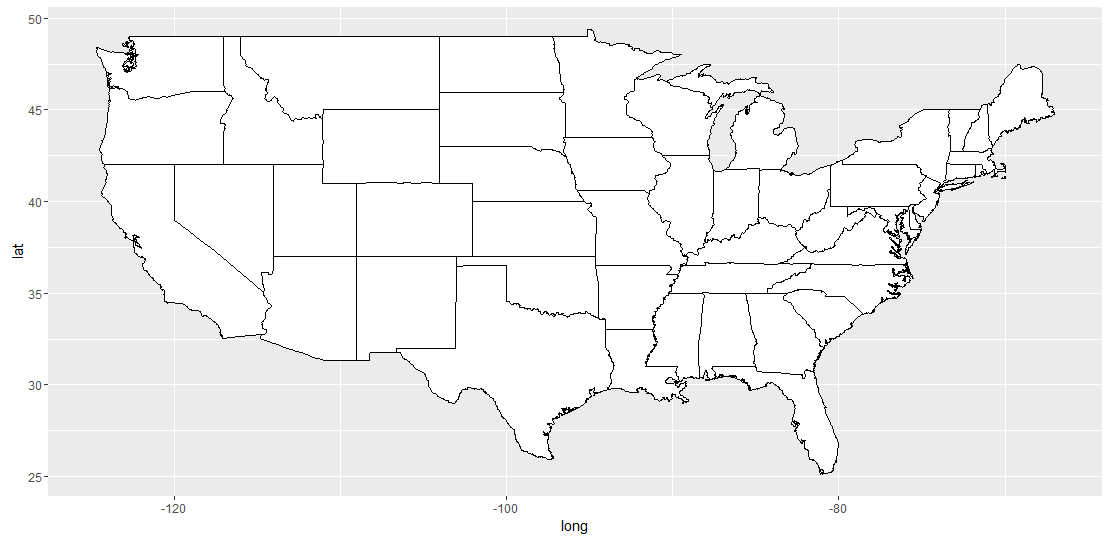
\includegraphics[width=.5\textwidth]{pictures/ggplot2/plainUSAmap.png} 
   \label{fig:plainUSAmap}
\end{figure} 

\noindent Now that could be useful for some things.
For example, maybe you want to
\begin{itemize}
    \item decorate your very own US map by hand
    \item memorize the locations of the lower 48 states (sorry Alaska and Hawaii)
\end{itemize}
But that's not what we're here to do.
Therefore, after you load some data, choose a few variables that you are interested in analysing.
If you are using the \texttt{state.x77} dataset from the datasets package, there are several to choose from other than income, including high school graduation rates, frost levels, and murder rates.
Once you have chosen your variables and written it into the code, you should output a chloropleth map that looks something like figure \ref{fig:OGUSAmap}.

\begin{figure}[htbp!]
   \centering
      \caption{Base Chloropleth USA Map}
   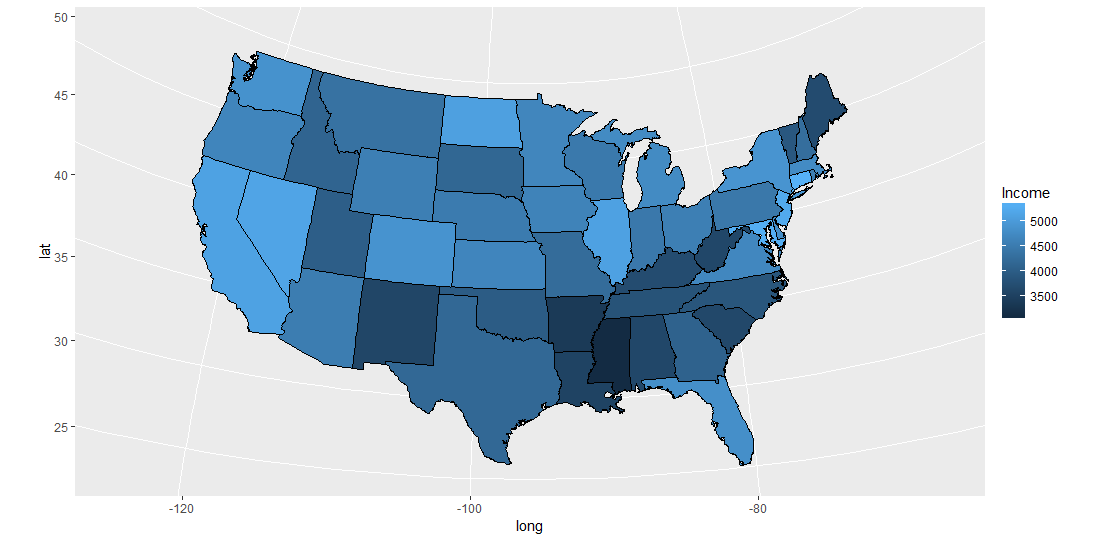
\includegraphics[width=0.5\textwidth]{pictures/ggplot2/OGUSAmap.png} 
   \label{fig:OGUSAmap}
\end{figure} 

Now we're getting somewhere! From there, you can customize it further by changing the background, state border outlines, gradient colors, and more.
For the example map, we chose to create a map with a plain background devoid of latitude and longitude lines plus a gradient that ranges from white to maroon.
You can see the result in figure \ref{fig:whitemaroonUSAmap}.

\begin{figure}[htbp!]
   \centering
      \caption{Final USA Chloropleth Map}
   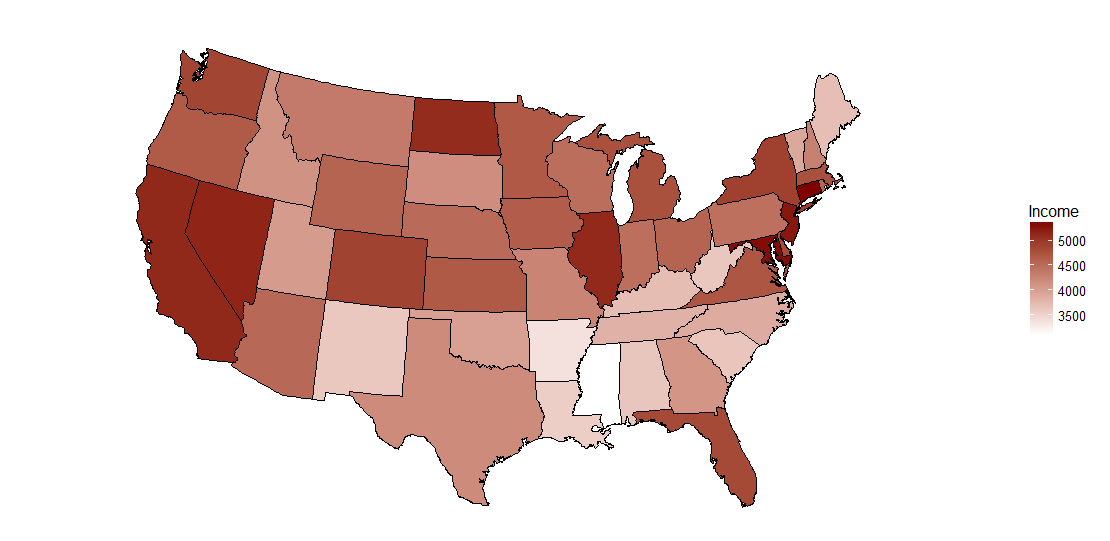
\includegraphics[width=0.5\textwidth]{pictures/ggplot2/whitemaroonUSAmap.png} 
   \label{fig:whitemaroonUSAmap}
\end{figure} 

 
\section{Deliverable}

The final product that you create should consist of two plots mapped with different colors that contain discrete variables, a scatter plot with a continuous variable mapped with a gradient, and a chloropleth map.

\section{Teaching Code}

\begin{lstlisting}

# Katherine L. Bennett
# October 15, 2016
# ggplot.R script
# This code outlines different ways to use ggplot2 to organize and
# color various plots and charts
#
# begin by cleaning your workspace and setting your working directory
rm(list = ls())
setwd("C:/Users/Katherine/Desktop/RFiles")
#
# install necessary packages
install.packages("ggplot2")
install.packages("gcookbook")
#
# load libraries
library(ggplot2)
library(gcookbook)
library(RColorBrewer)
#
# Now let's begin Objective 1
#
# download your dataset - I found mine from an online base (listed
# in bibliography), but gcookbook also has several good options
# load your data using the script window or import it directly 
# under the "Environment" tab
read.csv("uspopagegroup")
#
# this is your base plot
p <- ggplot(uspopagegroup, mapping = aes(x = Year, y = Population,
fill = AgeGroup)) + geom_area()
#
# the following 3 commands do the exact same thing and use the
# basic/default palette
p
p + scale_fill_hue()
p + scale_fill_discrete()
#
# you can change colors using different palettes
p + scale_fill_grey() # this one uses various greys
#
# the brewer palette has a huge range of color combinations
p + scale_fill_brewer() # this is the base Brewer palette, which
# uses a swath of blues
# to access the full range of Brewer palettes, use:
display.brewer.all() # look at all those colors!
# once you find a palette you like, simply include it in your
# command
p + scale_fill_brewer(palette = "OrRd")
#
# to specify your own color choices, you can use the manual option
p + scale_fill_manual(values = c("red", "green", "blue", "yellow"))
# this is a bit of an eye sore, but you get the idea
#
# try out another example of color-coding charts using a discrete
# variable
# download dataset - again, mine is from online, but you can find
# your own or use one from gcookbook
# load dataset
read.csv("Davis")
#
# begin with your base plot again
d <- ggplot(Davis, aes(x = weight, y = height, colour = sex)) +
geom_point()
d
#
# now the plot colored by sex; to change the colors, use different
# color values
# the same technique applied to the first dataset can also be
# applied to this one
d + scale_color_brewer(palette = "Oranges")
d + scale_color_manual(values = c("orange", "blue"))
# etc., etc.
#
#
# now we will begin Objective 2 - continuous variables
#
#
# load your dataset; this time, I found mine in the R "datasets"
# package
library(datasets)
#
# start with your base plot
m <- ggplot(mtcars, aes(x = wt, y = mpg, colour = disp)) +
geom_point(size = 7)
m
#
# here is a gradient that ranges between two colors
m + scale_colour_gradient(low = "black", high = "white")
#
# this is a gradient with a white midpoint
library(scales)
m + scale_colour_gradient2(low = "red", mid = "white", high =
"blue", midpoint = 250)
#
# lastly, here is a gradient with "n" number of gradient colors
m + scale_colour_gradientn(colours = c("darkgreen", "green",
"yellow", "white"))
#
#
# On to Objective 3!
#
#
# begin by loading the map library
library(maps)
# retrieve map data for USA
states_map <- map_data("state")
#
# start with a basic map of the US (I can feel those patriotic
# juices flowing!)
ggplot(states_map, aes(x = long, y = lat, group = group)) +
geom_polygon(fill = "white", colour = "black")
# so this map is a little boring right? Let's spice it up a bit by
# adding some data
#
# for this example, we're going to use some US income stats
#
# change the state.x77 dataset (included in the R datasets package)
# to the proper format
income <- data.frame(state = tolower(rownames(state.x77)),
state.x77)
income
#
# merge the datasets together
income_map <- merge(states_map, income, by.x = "region", by.y =
"state")
#
# sort the data
head(income_map)
library(plyr) # needed in order to use the arrange() function
# sort by group, then order
income_map <- arrange(income_map, group, order)
head(income_map)
#
# now plot your basic map
ggplot(lit_map, aes(x = long, y = lat, group = group, fill =
Income)) + 
  geom_polygon(colour = "black") + # this outlines the states in
  # black
  coord_map("polyconic")
# look how nice that is! Now let's add a personal touch...
#
# in order to create a blank, line free background, you can name 
# and use the following function:
theme_clean <- function(base_size = 12) {
  require(grid)
    theme_grey(base_size) %+replace%
      theme(
        axis.title = element_blank(),
        axis.text = element_blank(),
        panel.background = element_blank(),
        panel.grid = element_blank(),
        axis.ticks.length = unit(0, "cm"),
        panel.margin = unit(0, "lines"),
        plot.margin = unit(c(0, 0, 0, 0), "lines"),
        complete = TRUE
      )
}
#
# now to add some different colors and our new theme_clean() function 
# to the base plot
ggplot(lit_map, aes(x = long, y = lat, group = group, fill = Income)) + 
  geom_polygon(colour = "black") +
  scale_fill_gradient(low = "#FFFFFF", high = "#800000") +
  coord_map("polyconic") +
  theme_clean() # look at that nice map! Aren't you proud?
#
# I hope you enjoyed these exercises and good luck with all of your
# future coloring! At least now it's easier to keep it in the lines,
# right?
#
# End of code
\end{lstlisting}

\section{Example Student Code}

\begin{lstlisting}

# Katherine L. Bennett
# October 15, 2016
# ggplot.R script
# This code outlines different ways to use ggplot2 to organize and
# color various plots and charts
#
# clean workspace and set working directory
rm(list = ls())
setwd("C:/Users/Katherine/Desktop/RFiles")
#
# install packages
install.packages("ggplot2")
install.packages("gcookbook")
#
# load libraries
library(ggplot2)
library(gcookbook)
library(RColorBrewer)
#
# Objective 1
#
# Example 1
# load data
read.csv("uspopagegroup")
#
# this is your base plot
p <- ggplot(uspopagegroup, mapping = aes(x = Year, y = Population,
fill = AgeGroup)) + geom_area()
p
p + scale_fill_hue()
p + scale_fill_discrete()
#
# change colors using different palettes
p + scale_fill_grey()
p + scale_fill_brewer()
# access the full range of Brewer palettes
display.brewer.all() 
p + scale_fill_brewer(palette = "OrRd")
#
# specify own color choices
p + scale_fill_manual(values = c("red", "green", "blue", "yellow"))
#
# Example 2
# load dataset
read.csv("Davis")
#
# base plot
d <- ggplot(Davis, aes(x = weight, y = height, colour = sex)) +
geom_point()
d
#
# plot colored by sex
d + scale_color_brewer(palette = "Oranges")
d + scale_color_manual(values = c("orange", "blue"))
# etc., etc.
#
#
# Objective 2
#
#
# load data
library(datasets)
#
# start with your base plot
m <- ggplot(mtcars, aes(x = wt, y = mpg, colour = disp)) +
geom_point(size = 7)
m
#
# gradient that ranges between two colors
m + scale_colour_gradient(low = "black", high = "white")
#
# gradient with a white midpoint
library(scales)
m + scale_colour_gradient2(low = "red", mid = "white", high =
"blue", midpoint = 250)
#
# gradient with "n" number of colors
m + scale_colour_gradientn(colours = c("darkgreen", "green",
"yellow", "white"))
#
#
# Objective 3
#
#
# begin by loading the map library
library(maps)
# retrieve map data for USA
states_map <- map_data("state")
#
# basic US map
ggplot(states_map, aes(x = long, y = lat, group = group)) +
geom_polygon(fill = "white", colour = "black")
#
# change dataset to the proper format
income <- data.frame(state = tolower(rownames(state.x77)),
state.x77)
income
#
# merge the datasets together
income_map <- merge(states_map, income, by.x = "region", by.y =
"state")
#
# sort the data
head(income_map)
library(plyr)
# sort by group, then order
income_map <- arrange(income_map, group, order)
head(income_map)
#
# plot basic map
ggplot(lit_map, aes(x = long, y = lat, group = group, fill =
Income)) + 
  geom_polygon(colour = "black") + 
  coord_map("polyconic")
#
# clean up the background
theme_clean <- function(base_size = 12) {
  require(grid)
  theme_grey(base_size) %+replace%
    theme(
      axis.title = element_blank(),
      axis.text = element_blank(),
      panel.background = element_blank(),
      panel.grid = element_blank(),
      axis.ticks.length = unit(0, "cm"),
      panel.margin = unit(0, "lines"),
      plot.margin = unit(c(0, 0, 0, 0), "lines"),
      complete = TRUE
    )
}
#
# personalize/add final touches to base plot
ggplot(lit_map, aes(x = long, y = lat, group = group, fill =
Income)) + 
  geom_polygon(colour = "black") +
  scale_fill_gradient(low = "#FFFFFF", high = "#800000") +
  coord_map("polyconic") +
  theme_clean()
#
# End of code
\end{lstlisting}


\section{Further Readings}

\indent There is an endless supply of sources available that offer tips, tutorials, and exercises with ggplot2.
Winston Chang's \emph{GCookBook} is a personal favorite and was used to help create this very chapter.
It lists over 150 exercises designed to help you create charts and graphics even if you have little prior experience.
There is also a basic online version available at www.cookbook-r.com/Graphs/. \newline \newline \emph{ggplot2: Elegant Graphics for Data Analysis} by Hadley Wickham is another great reference if you want to better understand how all of the elements of ggplot2 fit together, which is ideal if you want to create graphics specifically tailored to your data and research.
\medskip

\noindent Lastly, Vanderbilt offered a workshop on ggplot2 that can be viewed here: \newline ggplot2.org/resources/2007-vanderbilt.pdf.
